\section{原始—对偶内点法}
\label{sec:nlipm-primal-dual}

障碍法有两个不便之处。一维例子已经显示，参数减小之后，从旧碗底出发的Newton步可能完全不可信。另外它要求每个迭代点都严格满足$\bm{g}(\bm{x})<\bm{0}$，弯的约束使这件事代价不小。于是要问：把乘子和松弛都当作独立变量，同时更新，能否绕开这两点，又要付出什么代价？

\subsection{扰动互补方程}
\label{sec:nlipm-perturbed}

方程组~\eqref{eq:nlipm-perturbed-kkt}里，$-g_i$既是约束值，又是互补方程的一个因子。引入\term{松弛变量}（slack variable）$\bm{s}\in\mathbb{R}^m$，把它们分开：
\begin{equation}
 \begin{aligned}
 \nabla f(\bm{x})+\bm{J}(\bm{x})^\top\bm{\lambda}+\bm{A}(\bm{x})^\top\bm{\nu}&=\bm{0},\\
 \bm{h}(\bm{x})&=\bm{0},\\
 \bm{g}(\bm{x})+\bm{s}&=\bm{0},\\
 s_i\lambda_i&=\mu\quad(i=1,\ldots,m),\\
 \bm{s}>\bm{0},\quad\bm{\lambda}&>\bm{0}.
 \end{aligned}
 \label{eq:nlipm-pd-system}
\end{equation}
这里的乘子$\bm{\lambda}$沿用第~\ref{chap:constrained-optimality}章的符号。要留意$\bm{s}$的角色变了：第~\ref{chap:lp-interior-point}章的$\bm{s}$是对偶松弛，这里的$\bm{s}$是原始松弛，对偶一侧的正变量是$\bm{\lambda}$。表~\ref{tab:nlipm-lp-correspondence}列出两章量的对应，取$\bm{g}(\bm{x})=-\bm{x}$就回到线性规划。

\begin{BookInlineTable}
  \centering
  \footnotesize
  \begin{tabular}{@{}lll@{}}
    \toprule
    量 & 线性规划 & 一般约束\\
    \midrule
    原始侧的正变量 & $\bm{x}$ & $\bm{s}=-\bm{g}(\bm{x})$\\
    对偶侧的正变量 & $\bm{s}$ & $\bm{\lambda}$\\
    扰动互补 & $x_is_i=\mu$ & $s_i\lambda_i=\mu$\\
    不等式约束数 & $n$ & $m$\\
    Jacobian & $-\bm{I}$，常数 & $\bm{J}(\bm{x})$，随点变化\\
    等式的Jacobian & $\bm{A}$，常数 & $\bm{A}(\bm{x})$，随点变化\\
    二阶信息 & 无 & Lagrange Hessian\\
    \bottomrule
  \end{tabular}
  \caption{线性规划内点法与一般约束内点法中各量的对应。}
  \label{tab:nlipm-lp-correspondence}
\end{BookInlineTable}

\paragraph{正性和参数各管什么}
方程组~\eqref{eq:nlipm-pd-system}有两类要求，作用不同。$\bm{s},\bm{\lambda}>\bm{0}$是内部性，它不是方程，而是对解的筛选。$\mu>0$是中心性，它要求所有乘积相等，从而把组合选择（哪个因子为零）换成一条光滑的曲线。

去掉正性，方程会多出不该要的解。回到一维例子$\min x$、$x^2-1\leq0$，方程组是
\[
 1+2\lambda x=0,\qquad x^2-1+s=0,\qquad s\lambda=\mu.
\]
消去$\lambda$和$s$，得到$1-x^2+2\mu x=0$，它有两个根$x=\mu\pm\sqrt{\mu^2+1}$。

取$\mu=3/4$。根$x=-1/2$给出$s=3/4$、$\lambda=1$，这是碗底。根$x=2$给出
\[
 s=-3,\qquad\lambda=-\frac14,\qquad s\lambda=\frac34.
\]
方程全部满足，两个因子却都是负的，这个点在可行域之外。$\mu\to0$时它趋于$x=1$，那是原问题的最大点。所以正性不是可有可无的附加条件，它把算法挡在对的那一支上。

\paragraph{残差小、乘积小和已经最优是三回事}
方程组~\eqref{eq:nlipm-pd-system}令人误以为只要把某个量压小就算成功。在贯穿例的点$\bm{x}=(1,2)^\top$、$\bm{s}=(1,2)^\top$上看两种选择。

第一种取$\bm{\lambda}=(10^{-3},10^{-3})^\top$。这时松弛方程精确满足，两个乘积分别是$10^{-3}$和$2\times10^{-3}$，都很小，驻定残差却是
\[
 \nabla f+\bm{J}^\top\bm{\lambda}\approx(-1.998,\,2)^\top,
\]
离$\bm{0}$很远。互补小，只说明$s_i\lambda_i$小，不说明点接近最优。

第二种取$\mu=1$的中心点。这时所有方程残差都是零，乘积却等于$1$。残差为零说明的是“解对了当前的$\mu$”，而不是解对了原问题。只有方程残差和互补量同时小，才接近KKT点。在非凸问题上，即便接近KKT点，也还要另外判断它是不是极小点。

\subsection{Newton方向}
\label{sec:nlipm-newton}

\paragraph{主要思想：线性化扰动方程}
当前点记为$(\bm{x},\bm{s},\bm{\lambda},\bm{\nu})$，只要求$\bm{s},\bm{\lambda}>\bm{0}$。平均互补量和本轮的目标参数是
\begin{equation}
 \mu=\frac{\bm{s}^\top\bm{\lambda}}{m},\qquad\hat{\mu}=\sigma\mu,\quad\sigma\in[0,1).
 \label{eq:nlipm-mu}
\end{equation}
定义四个残差，它们分别度量驻定、等式、松弛方程和互补目标还差多少：
\begin{equation}
 \begin{aligned}
 \bm{r}_{\mathrm{d}}&=\nabla f(\bm{x})+\bm{J}(\bm{x})^\top\bm{\lambda}+\bm{A}(\bm{x})^\top\bm{\nu},\\
 \bm{r}_{\mathrm{e}}&=\bm{h}(\bm{x}),\qquad
 \bm{r}_{\mathrm{p}}=\bm{g}(\bm{x})+\bm{s},\\
 \bm{r}_{\mathrm{c}}&=\hat{\mu}\bm{1}-\bm{S}\bm{\Lambda}\bm{1},
 \end{aligned}
 \label{eq:nlipm-residuals}
\end{equation}
其中$\bm{S}=\operatorname{diag}(\bm{s})$，$\bm{\Lambda}=\operatorname{diag}(\bm{\lambda})$。

对方程组作Newton线性化，需要各方程对变量的导数。第一个方程对$\bm{x}$求导，得到\term{Lagrange Hessian}（Lagrangian Hessian）
\begin{equation}
 \bm{W}=\nabla^2f(\bm{x})+\sum_{i=1}^m\lambda_i\nabla^2g_i(\bm{x})+\sum_{j=1}^p\nu_j\nabla^2h_j(\bm{x}),
 \label{eq:nlipm-lagrange-hessian}
\end{equation}

对$\bm{\lambda}$、$\bm{\nu}$求导得到$\bm{J}^\top$、$\bm{A}^\top$。其余方程的导数可以直接读出。于是方向由下面的线性方程组确定：
\begin{equation}
 \begin{bmatrix}
 \bm{W}&\bm{0}&\bm{J}^\top&\bm{A}^\top\\
 \bm{J}&\bm{I}&\bm{0}&\bm{0}\\
 \bm{A}&\bm{0}&\bm{0}&\bm{0}\\
 \bm{0}&\bm{\Lambda}&\bm{S}&\bm{0}
 \end{bmatrix}
 \begin{bmatrix}\Delta\bm{x}\\\Delta\bm{s}\\\Delta\bm{\lambda}\\\Delta\bm{\nu}\end{bmatrix}
 =
 \begin{bmatrix}-\bm{r}_{\mathrm{d}}\\-\bm{r}_{\mathrm{p}}\\-\bm{r}_{\mathrm{e}}\\\bm{r}_{\mathrm{c}}\end{bmatrix}.
 \label{eq:nlipm-newton}
\end{equation}
和第~\ref{chap:lp-interior-point}章的方程组比较，第四行结构不变，新增的是左上角的$\bm{W}$，以及$\bm{J}$、$\bm{A}$每轮都要重新计算。线性规划中$\bm{W}=\bm{0}$。

\paragraph{消元与鞍点结构}
图~\ref{fig:nlipm-kkt-blocks}是消元的路线。由第二行，松弛的方向是
\begin{equation}
 \Delta\bm{s}=-\bm{r}_{\mathrm{p}}-\bm{J}\Delta\bm{x}.
 \label{eq:nlipm-ds}
\end{equation}
由第四行，乘子的方向是
\begin{equation}
 \Delta\bm{\lambda}=\bm{S}^{-1}\bigl(\bm{r}_{\mathrm{c}}-\bm{\Lambda}\Delta\bm{s}\bigr).
 \label{eq:nlipm-dlambda}
\end{equation}

\begin{BookInlineFigure}
  \centering
  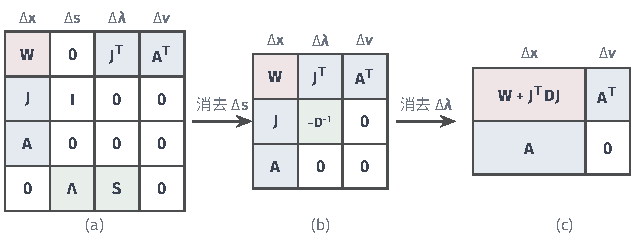
\includegraphics[width=107.5mm]{figures/05-optimization/06-constrained-optimization/tikz/nlipm-kkt-blocks/figure.pdf}
  \caption{Newton方程组的三种等价形式，顶部标出每列对应的方向。红底是含曲率的块，蓝底是约束Jacobian，绿底是对角块，$\bm{D}=\bm{S}^{-1}\bm{\Lambda}$。(a)式~\eqref{eq:nlipm-newton}；(b)消去$\Delta\bm{s}$后的对称鞍点形式；(c)再消去$\Delta\bm{\lambda}$后的压缩形式。}
  \label{fig:nlipm-kkt-blocks}
\end{BookInlineFigure}

把式~\eqref{eq:nlipm-ds}代入式~\eqref{eq:nlipm-dlambda}，再代入第一行，$\Delta\bm{\lambda}$被消去，只剩$\Delta\bm{x}$和$\Delta\bm{\nu}$。记对角矩阵$\bm{D}=\bm{S}^{-1}\bm{\Lambda}$，以及
\begin{equation}
 \tilde{\bm{H}}=\bm{W}+\bm{J}^\top\bm{D}\bm{J},\qquad
 \bm{b}=-\bm{r}_{\mathrm{d}}-\bm{J}^\top\bm{S}^{-1}\bigl(\bm{r}_{\mathrm{c}}+\bm{\Lambda}\bm{r}_{\mathrm{p}}\bigr).
 \label{eq:nlipm-condensed-data}
\end{equation}
方向$\Delta\bm{x}$、$\Delta\bm{\nu}$满足压缩后的鞍点方程
\begin{equation}
 \begin{bmatrix}\tilde{\bm{H}}&\bm{A}^\top\\\bm{A}&\bm{0}\end{bmatrix}
 \begin{bmatrix}\Delta\bm{x}\\\Delta\bm{\nu}\end{bmatrix}
 =\begin{bmatrix}\bm{b}\\-\bm{r}_{\mathrm{e}}\end{bmatrix}.
 \label{eq:nlipm-condensed}
\end{equation}

$\tilde{\bm{H}}$的两部分对应障碍的两种作用：$\bm{J}^\top\bm{D}\bm{J}$在约束法向上加刚度，$\bm{W}$保留目标和约束的弯曲。在式~\eqref{eq:nlipm-newton}的第二种写法里，只消去$\Delta\bm{s}$，保留$\Delta\bm{\lambda}$，得到的矩阵是
\begin{equation}
 \begin{bmatrix}\bm{W}&\bm{J}^\top&\bm{A}^\top\\\bm{J}&-\bm{D}^{-1}&\bm{0}\\\bm{A}&\bm{0}&\bm{0}\end{bmatrix}.
 \label{eq:nlipm-saddle}
\end{equation}
压缩形式维数小，鞍点形式稀疏性好，第~\ref{sec:nlipm-guarantees}节比较它们的代价。

举一个带等式约束的算例，看$\bm{A}$的作用。取下面的矩阵$\tilde{\bm{H}}$和右端$\bm{b}$（稍后的计算过程会在贯穿例的第一轮得到它们），再加一条等式约束$x_1-x_2+1=0$，当前点$(1,2)$满足它，所以$r_{\mathrm{e}}=0$：
\[
 \tilde{\bm{H}}=\begin{bmatrix}7&-2\\-2&9/4\end{bmatrix},\qquad\bm{b}=\begin{bmatrix}8/5\\-19/10\end{bmatrix},\qquad\bm{A}=[1\ \ -1].
\]
由$\bm{A}\Delta\bm{x}=0$，方向只能取$\Delta\bm{x}=\tau(1,1)^\top$。用$(1,1)$左乘第一块方程，$\Delta\nu$相互抵消，得到
\[
 \tfrac{21}{4}\tau=-\tfrac{3}{10},\qquad\text{即}\qquad\tau=-\frac{2}{35}.
\]
再由第一行，$5\tau+\Delta\nu=8/5$，于是$\Delta\nu=66/35$。等式约束的作用是把方向压进切平面，这和第~\ref{chap:quadratic-conic-programming}章的等式约束二次规划一样。

\paragraph{与障碍法的Newton方向比较}
若$\bm{s}=-\bm{g}(\bm{x})$，$\bm{\lambda}=\mu\bm{S}^{-1}\bm{1}$，则$\tilde{\bm{H}}=\nabla^2B_\mu$，两种方法在这一点上的矩阵相同。差别出现在其他点：参数一降，障碍法的乘子估计立刻变成$\mu^+/s_i$，原始—对偶方法的$\lambda_i$则留在当前值，由方程去修正。

回到一维例子，站在$x=-1/2$、$s=3/4$、$\lambda=1$，目标参数$\hat{\mu}=0.05$。这时
\[
 W=2,\quad J=-1,\quad D=\frac43,\quad\tilde{H}=\frac{10}{3},\quad r_{\mathrm{c}}=0.05-0.75=-0.7.
\]
由式~\eqref{eq:nlipm-condensed-data}，$b=-J\,r_{\mathrm{c}}/s=-14/15$，于是
\[
 \Delta x=-0.28,\qquad\Delta s=-0.28,\qquad\Delta\lambda=-0.56.
\]
单位步得到$x=-0.78$、$s=0.47$、$\lambda=0.44$，都留在正确的一侧。同样的起点和目标参数，障碍法的Newton步是$-4.2$。这里的差别和第~\ref{chap:lp-interior-point}章线性化$x_is_i=\mu$而不线性化$s_i=\mu/x_i$是同一个原因。

\paragraph{曲率让残差不再按比例下降}
线性规划中，走步长$\alpha$后等式残差精确地乘以$1-\alpha$。这个性质来自约束是线性的。现在对松弛方程作Taylor展开，走完步长$\alpha$，残差变成
\begin{equation}
 \bm{r}_{\mathrm{p}}^+=(1-\alpha)\bm{r}_{\mathrm{p}}+\bm{\rho}(\alpha),
 \label{eq:nlipm-rp-update}
\end{equation}
其中二阶余项是
\[
 \bm{\rho}(\alpha)=\bm{g}(\bm{x}+\alpha\Delta\bm{x})-\bm{g}(\bm{x})-\alpha\bm{J}\Delta\bm{x}.
\]
若$\nabla g_i$是$L_g$-Lipschitz的，则余项的大小满足
\[
 \lvert\rho_i(\alpha)\rvert\leq\tfrac12L_g\alpha^2\lVert\Delta\bm{x}\rVert_2^2.
\]

贯穿例的$g_1=x_1^2-x_2$是二次的，余项可以精确写出：
\[
 \rho_1(\alpha)=\alpha^2\Delta x_1^2.
\]
图~\ref{fig:nlipm-curved-residual}取一个可行域外的点。线性模型认为约束边界是黄色的切线，走完单位步正好到达；实际约束是抛物线，单位步之后的残差不是零，而是$\Delta x_1^2\approx0.746$。

这个现象还有一个后果：即使当前点满足$\bm{r}_{\mathrm{p}}=\bm{0}$，走一步后也可能变成非零。原始可行性在线性规划中可以一旦达到就永远保持，这里不能。

\begin{BookInlineFigure}
  \centering
  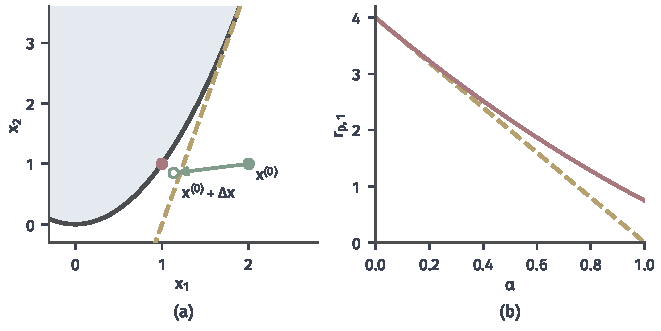
\includegraphics[width=112mm]{figures/05-optimization/06-constrained-optimization/matplotlib/nlipm-curved-residual/figure.pdf}
  \caption{弯的约束使线性化产生误差，贯穿例，起点$\bm{x}^{(0)}=(2,1)$、$\bm{s}=(1,3)$、$\bm{\lambda}=(1,1/3)$、$\sigma=0.2$。(a)深灰粗线是真实边界，黄色虚线是在$\bm{x}^{(0)}$处线性化的边界，绿色箭头是Newton步，红点是$\bm{x}^\star$。(b)红线是实际残差$r_{\mathrm{p},1}$，黄色虚线是线性模型预测的$(1-\alpha)r_{\mathrm{p},1}$，$\alpha=1$时两者相差$\Delta x_1^2$。}
  \label{fig:nlipm-curved-residual}
\end{BookInlineFigure}

\paragraph{线性系统可解，不等于方向好用}
方程组~\eqref{eq:nlipm-condensed}何时有唯一解，答案和约化Hessian有关。

\begin{lemma}[Newton方程的解]
\label{lem:nlipm-newton-solvable}
设$\bm{s},\bm{\lambda}>\bm{0}$，$\bm{A}$满行秩，$\tilde{\bm{H}}$在$\bm{A}$的零空间上正定，即$\bm{A}\bm{d}=\bm{0}$、$\bm{d}\neq\bm{0}$时$\bm{d}^\top\tilde{\bm{H}}\bm{d}>0$。则方程组~\eqref{eq:nlipm-newton}有唯一解。
\end{lemma}

\begin{proof}
消元的每一步都是等价变形，所以只需证明压缩矩阵非奇异。设
\[
 \tilde{\bm{H}}\bm{d}+\bm{A}^\top\bm{w}=\bm{0},\qquad\bm{A}\bm{d}=\bm{0}.
\]
用$\bm{d}^\top$左乘第一式，并用第二式，得到
\[
 \bm{d}^\top\tilde{\bm{H}}\bm{d}=0.
\]
由正定性$\bm{d}=\bm{0}$。于是$\bm{A}^\top\bm{w}=\bm{0}$，由满行秩$\bm{w}=\bm{0}$。
\end{proof}

这个条件比“系数矩阵非奇异”强。矩阵非奇异时方程也有唯一解，但方向可能完全不对。下面的引理说明正定性的真正用途：它保证方向使障碍目标下降。这里的障碍目标把松弛也当作变量，写成
\[
 \psi_{\hat{\mu}}(\bm{x},\bm{s})=f(\bm{x})-\hat{\mu}\sum_{i=1}^m\log s_i.
\]

\begin{lemma}[方向与障碍目标]
\label{lem:nlipm-descent}
设$\bm{r}_{\mathrm{p}}=\bm{0}$，$\bm{r}_{\mathrm{e}}=\bm{0}$，方向由式~\eqref{eq:nlipm-newton}给出，其中目标参数取$\hat{\mu}$。则$\psi_{\hat{\mu}}$沿方向的一阶变化满足
\begin{equation}
 \nabla f^\top\Delta\bm{x}-\hat{\mu}\,\bm{1}^\top\bm{S}^{-1}\Delta\bm{s}=-\Delta\bm{x}^\top\tilde{\bm{H}}\Delta\bm{x}.
 \label{eq:nlipm-descent}
\end{equation}
\end{lemma}

\begin{proof}
由$\bm{r}_{\mathrm{d}}$的定义和$\bm{A}\Delta\bm{x}=\bm{0}$、$\bm{J}\Delta\bm{x}=-\Delta\bm{s}$，有
\[
 \nabla f^\top\Delta\bm{x}=\bm{r}_{\mathrm{d}}^\top\Delta\bm{x}+\bm{\lambda}^\top\Delta\bm{s}.
\]
互补残差满足
\[
 \bm{S}^{-1}\bm{r}_{\mathrm{c}}=\hat{\mu}\bm{S}^{-1}\bm{1}-\bm{\lambda}.
\]
用$\Delta\bm{x}^\top$左乘式~\eqref{eq:nlipm-condensed}的第一块，并代入上式，得到
\[
 \Delta\bm{x}^\top\tilde{\bm{H}}\Delta\bm{x}=-\bm{r}_{\mathrm{d}}^\top\Delta\bm{x}+(\hat{\mu}\bm{S}^{-1}\bm{1}-\bm{\lambda})^\top\Delta\bm{s}.
\]
由第二式解出$\bm{r}_{\mathrm{d}}^\top\Delta\bm{x}$，代入第一式，$\bm{\lambda}^\top\Delta\bm{s}$相互抵消，即得结论。
\end{proof}

所以$\tilde{\bm{H}}$在切空间上不正定时，$\Delta\bm{x}$可能是上升方向。图~\ref{fig:nlipm-regularization}取圆盘外部的例子，$\mu=0.1$，在$\bm{x}=(0.35,1.08)^\top$处的特征值是
\[
 -0.320,\qquad 7.352.
\]
Newton方向的一阶变化是$\nabla B_\mu^\top\bm{d}=+0.947$，它是上升方向，指向鞍点。系数矩阵非奇异，线性方程解得毫无困难，得到的却是错误的方向。

补救办法是\term{矩阵正则化}（matrix regularization）：把$\tilde{\bm{H}}$换成$\tilde{\bm{H}}+\delta_{\mathrm{w}}\bm{I}$，$\delta_{\mathrm{w}}\geq0$逐步增大，直到切空间上正定。例中取$\delta_{\mathrm{w}}=0.47$，新方向的一阶变化是$-2.73$，变成下降方向。

怎样判断切空间上正定？实际中不直接算切空间，而看鞍点矩阵的惯性，即正、负、零特征值的个数。$\bm{A}$满行秩时，$\tilde{\bm{H}}$在零空间上正定，当且仅当矩阵~\eqref{eq:nlipm-condensed}的惯性是$(n,p,0)$。分解$\bm{L}\bm{D}\bm{L}^\top$时可以直接读出惯性，所以试探$\delta_{\mathrm{w}}$只要重复分解。这个判据的证明要用到Sylvester惯性定律，读者可查阅专著\scite{math-nocedal2006numerical}。

\begin{BookInlineFigure}
  \centering
  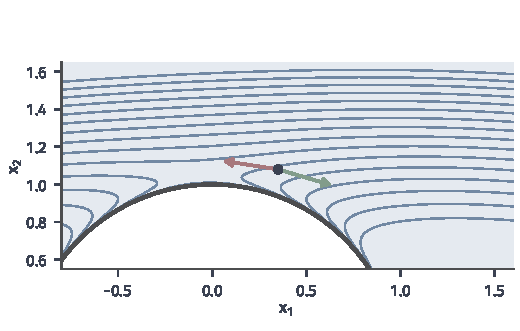
\includegraphics[width=88mm]{figures/05-optimization/06-constrained-optimization/matplotlib/nlipm-regularization/figure.pdf}
  \caption{曲率不定时的方向，圆盘外部的例子，$\mu=0.1$。深灰粗线是约束边界，蓝线是$B_\mu$的等值线，黑点是当前点。红色箭头是未修正的Newton方向，指向上升一侧的鞍点（为便于观察，按比例缩短）；绿色箭头是加上$\delta_{\mathrm{w}}\bm{I}$之后的方向，沿下降方向走向右侧的极小点。}
  \label{fig:nlipm-regularization}
\end{BookInlineFigure}

另一类困难来自约束退化。若活动约束或等式约束的梯度线性相关，$\bm{A}$不再满行秩，矩阵奇异或接近奇异。常用的办法是在右下角加上$-\delta_{\mathrm{c}}\bm{I}$，相当于允许等式约束有微小的违反。数值尺度也要处理：把某条约束乘以$1000$，$\bm{D}$和残差的数值都跟着变，通常先对目标和约束的梯度作缩放。这些修改的代价是方向不再是真正的Newton方向，第~\ref{sec:nlipm-stopping}小节会说明为什么最后要按未经修改的问题检查结果。

\subsection{步长与中心性}
\label{sec:nlipm-step}

得到方向后，还要回答走多远。这里有三件事彼此独立：不能越过边界，这一步要确实有进展，迭代点不能离路径太远。

\paragraph{到边界的比例规则}
第一件事沿用第~\ref{chap:lp-interior-point}章的做法，只是作用在$(\bm{s},\bm{\lambda})$上：
\begin{equation}
 \alpha_{\max}=\min\Bigl\{\min_{\Delta s_i<0}\frac{s_i}{-\Delta s_i},\ \min_{\Delta\lambda_i<0}\frac{\lambda_i}{-\Delta\lambda_i}\Bigr\},\qquad
 \alpha=\min\{1,\ \eta\,\alpha_{\max}\},
 \label{eq:nlipm-alpha}
\end{equation}
其中$\eta\in(0,1)$，没有负分量时约定$\alpha_{\max}=+\infty$。

这条规则保护的是$\bm{s}>\bm{0}$，而不是$\bm{g}(\bm{x})<\bm{0}$。当$\bm{r}_{\mathrm{p}}\neq\bm{0}$时，$\bm{x}$可以暂时越过约束边界。这是原始—对偶方法相对于障碍法的自由，也是第~\ref{sec:nlipm-stopping}小节必须检查原约束的原因。

实现中常对原始变量和对偶变量用不同的步长，因为线性规划中“单一步长让互补量精确下降”的理由在这里已经不成立。下面的算例为了便于手算，仍用单一步长。

\paragraph{残差检验}
满足比例规则的步长仍可能太长，因为式~\eqref{eq:nlipm-rp-update}的余项和$\bm{W}$的变化都没有进入线性模型。最直接的检验是看方程残差有没有变小。把方程组写成$\bm{F}_{\hat{\mu}}(\bm{z})=\bm{0}$，其中$\bm{z}=(\bm{x},\bm{s},\bm{\lambda},\bm{\nu})$，要求
\begin{equation}
 \lVert\bm{F}_{\hat{\mu}}(\bm{z}+\alpha\Delta\bm{z})\rVert_2\leq(1-c\,\alpha)\lVert\bm{F}_{\hat{\mu}}(\bm{z})\rVert_2,
 \label{eq:nlipm-residual-armijo}
\end{equation}
其中$c\in(0,1)$是小常数，不满足时把$\alpha$减半。

\begin{lemma}[Newton方向使残差下降]
\label{lem:nlipm-residual-descent}
设$\bm{F}_{\hat{\mu}}$连续可微，其Jacobian矩阵在$\bm{z}$处非奇异，$\Delta\bm{z}$是Newton方向，$\bm{F}_{\hat{\mu}}(\bm{z})\neq\bm{0}$。则$\alpha>0$足够小时，式~\eqref{eq:nlipm-residual-armijo}成立。
\end{lemma}

\begin{proof}
记
\[
 \Theta(\alpha)=\tfrac12\lVert\bm{F}_{\hat{\mu}}(\bm{z}+\alpha\Delta\bm{z})\rVert_2^2.
\]
由Newton方程$\bm{G}\Delta\bm{z}=-\bm{F}$，其中$\bm{G}$是Jacobian矩阵，有
\[
 \Theta'(0)=\bm{F}^\top\bm{G}\Delta\bm{z}=-\lVert\bm{F}\rVert_2^2.
\]
于是残差范数的展开是
\[
 \sqrt{2\Theta(\alpha)}=\lVert\bm{F}\rVert_2(1-\alpha)+o(\alpha).
\]
而$c<1$，所以$\alpha$足够小时不等式成立。
\end{proof}

这个检验简单，但有明显的盲区：它只看方程残差，分不清极小点和鞍点。方程组的任何解都能把它压到零，包括前面的$x=2$（若不靠正性挡住）和各种局部极大点。所以在非凸问题上，更常用的检验还要看目标。

\paragraph{过滤器}
一个直接想法是把约束违反量和障碍目标合成一个数，用它来比较。这需要一个权重，取大了算法只管可行，取小了只管目标。\term{过滤器}（filter）绕开这个权重，它把每一步看成二维平面上的一个点：
\begin{equation}
 \theta(\bm{z})=\bigl\lVert(\bm{h}(\bm{x}),\ \bm{g}(\bm{x})+\bm{s})\bigr\rVert_2,\qquad
 \psi_\mu(\bm{x},\bm{s})=f(\bm{x})-\mu\sum_{i=1}^m\log s_i.
 \label{eq:nlipm-filter-pair}
\end{equation}

算法保存一些历史点$(\theta_l,\psi_l)$，试探点只要不被其中任何一个点支配，就可以接受，也就是对每个$l$，要么$\theta$比$\theta_l$小，要么$\psi_\mu$比$\psi_l$小。图~\ref{fig:nlipm-filter}中有三个历史点$(0.2,4)$、$(0.5,3)$、$(1,2.5)$。

试探点A$=(0.3,3.2)$的$\theta$比$(0.5,3)$和$(1,2.5)$都小，$\psi_\mu$又比$(0.2,4)$小，所以被接受。试探点B$=(0.6,3.5)$的两个分量都比$(0.5,3)$差，被拒绝。两项指标各有高低的点互不否定，两项都差的点才被淘汰。

实际的过滤器要求有一定幅度的改进，例如$\theta\leq(1-\gamma_\theta)\theta_l$或$\psi_\mu\leq\psi_l-\gamma_\psi\theta_l$，否则可能无穷地接受改进极小的点。如果步长被缩到极小仍不能接受，算法转入\term{可行性恢复}（feasibility restoration）阶段，暂时放下目标，只减小$\theta$。

\begin{BookInlineFigure}
  \centering
  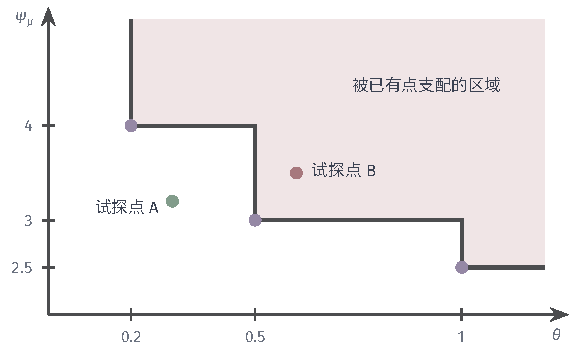
\includegraphics[width=97mm]{figures/05-optimization/06-constrained-optimization/tikz/nlipm-filter/figure.pdf}
  \caption{过滤器。横轴是约束违反量$\theta$，纵轴是障碍目标$\psi_\mu$。紫点是已保存的历史点，红底是被它们支配的区域。绿点A不被任何历史点支配，可以接受；红点B落在被支配区域内，被拒绝。}
  \label{fig:nlipm-filter}
\end{BookInlineFigure}

\paragraph{保持正性与靠近中心是两回事}
到边界的比例规则只保证$s_i,\lambda_i>0$。点可以严格在内部，却让某个乘积比平均值小几千倍，这时下一轮的Newton步很可能被这个小乘积卡住。沿用第~\ref{chap:lp-interior-point}章的度量，定义中心性
\begin{equation}
 \xi=\frac{\min_is_i\lambda_i}{\mu}\in(0,1].
 \label{eq:nlipm-centrality}
\end{equation}
要求$\xi\geq\gamma$（例如$\gamma=10^{-3}$）的集合称为\term{宽邻域}（wide neighborhood）。

图~\ref{fig:nlipm-wspace}把贯穿例的迭代画在$(s_1\lambda_1,s_2\lambda_2)$平面上。中心路径在这个平面上是对角线。绿线取$\sigma=0.2$，$\eta=0.9$，轨迹贴着对角线，中心性最低为$0.49$。

黄线取$\sigma=0.02$，$\eta=0.9999$，每步都几乎走到边界，第一步就让中心性掉到$10^{-3}$，再走两轮才恢复到$0.9$以上。正性两条线都保持了，靠近中心的程度却差别很大。

\begin{BookInlineFigure}
  \centering
  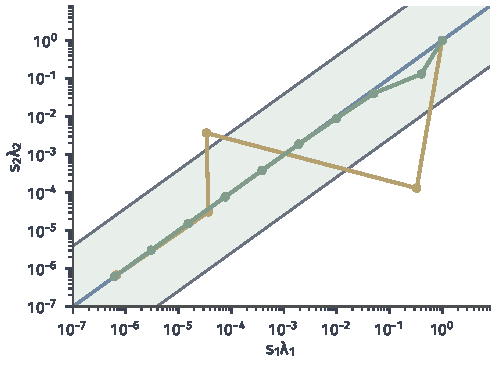
\includegraphics[width=84mm]{figures/05-optimization/06-constrained-optimization/matplotlib/nlipm-wspace/figure.pdf}
  \caption{互补乘积平面，对数坐标，贯穿例。蓝线是$s_1\lambda_1=s_2\lambda_2$，即中心路径；浅绿带是宽邻域$\xi\geq0.05$，灰线是其边界。绿线是$\sigma=0.2$、$\eta=0.9$的迭代，黄线是$\sigma=0.02$、$\eta=0.9999$的迭代，后者离开了浅绿带。}
  \label{fig:nlipm-wspace}
\end{BookInlineFigure}

\paragraph{计算过程}
下面把一轮迭代写成具体步骤，并在例~\eqref{eq:nlipm-running}上逐轮计算。取固定的中心化参数$\sigma=0.2$、比例$\eta=0.9$、残差检验常数$c=10^{-4}$，容差$\varepsilon=10^{-6}$。例中没有等式约束，含$\bm{A}$、$\bm{\nu}$的量都不出现。

\needspace{6\baselineskip}
\paragraph{变量}
\begin{itemize}
 \item $\bm{x}\in\mathbb{R}^n$：原始变量。$\bm{s}\in\mathbb{R}^m$：松弛，全部分量为正。
 \item $\bm{\lambda}\in\mathbb{R}^m$：不等式乘子，全部分量为正。$\bm{\nu}\in\mathbb{R}^p$：等式乘子。
 \item $\mu$、$\hat{\mu}$：平均互补量和本轮的目标参数，由式~\eqref{eq:nlipm-mu}给出。
 \item $\bm{r}_{\mathrm{d}},\bm{r}_{\mathrm{e}},\bm{r}_{\mathrm{p}},\bm{r}_{\mathrm{c}}$：式~\eqref{eq:nlipm-residuals}的四个残差，维数依次是$n$、$p$、$m$、$m$。
 \item $\bm{W}$、$\bm{D}$、$\tilde{\bm{H}}$、$\bm{b}$：Lagrange Hessian、对角缩放、压缩矩阵和右端，分别由式~\eqref{eq:nlipm-lagrange-hessian}、\eqref{eq:nlipm-condensed-data}给出。
 \item $\Delta\bm{x},\Delta\bm{s},\Delta\bm{\lambda},\Delta\bm{\nu}$：本轮的方向；$\alpha_{\max},\alpha$：最大步长和实际步长。
\end{itemize}

\paragraph{初始化}
取$\bm{x}^{(0)}$、$\bm{s}^{(0)}>\bm{0}$、$\bm{\lambda}^{(0)}>\bm{0}$和$\bm{\nu}^{(0)}$，令$t=0$；起点的选取由下一节讨论。例中取严格可行的点，并让两个乘积相等：
\[
 \bm{x}^{(0)}=\begin{bmatrix}1\\2\end{bmatrix},\qquad
 \bm{s}^{(0)}=-\bm{g}(\bm{x}^{(0)})=\begin{bmatrix}1\\2\end{bmatrix},\qquad
 \bm{\lambda}^{(0)}=\begin{bmatrix}1\\1/2\end{bmatrix}.
\]

\needspace{6\baselineskip}
\paragraph{每轮更新}
在第$t$轮，以$(\bm{x}^{(t)},\bm{s}^{(t)},\bm{\lambda}^{(t)},\bm{\nu}^{(t)})$为当前点：
\begin{enumerate}
 \item \textbf{计算残差并检查停止。}按式~\eqref{eq:nlipm-mu}、\eqref{eq:nlipm-residuals}计算$\mu$和残差。若$\lVert\bm{r}_{\mathrm{d}}\rVert_\infty$、$\lVert\bm{r}_{\mathrm{e}}\rVert_\infty$、$\lVert\bm{r}_{\mathrm{p}}\rVert_\infty$和$\max_is_i\lambda_i$都不超过$\varepsilon$，停止并输出当前点。

 例中第一轮$\mu^{(0)}=1$，$\hat{\mu}=0.2$，
 \[
  \bm{r}_{\mathrm{d}}=\begin{bmatrix}-2\\2\end{bmatrix}+\begin{bmatrix}2\\-1/2\end{bmatrix}=\begin{bmatrix}0\\3/2\end{bmatrix},\quad
  \bm{r}_{\mathrm{p}}=\bm{0},\quad
  \bm{r}_{\mathrm{c}}=\begin{bmatrix}-4/5\\-4/5\end{bmatrix}.
 \]

 \item \textbf{形成压缩方程。}由式~\eqref{eq:nlipm-lagrange-hessian}计算$\bm{W}$，由式~\eqref{eq:nlipm-condensed-data}计算$\tilde{\bm{H}}$和$\bm{b}$。检查惯性，必要时加$\delta_{\mathrm{w}}\bm{I}$。

 例中第一轮$\lambda_1=1$，所以$\bm{W}=\operatorname{diag}(3,1)$，而$\bm{D}=\operatorname{diag}(1,1/4)$，$\bm{J}$的两行是$(2,-1)$和$(0,1)$，所以
 \[
  \tilde{\bm{H}}=\begin{bmatrix}3&0\\0&1\end{bmatrix}+\begin{bmatrix}4&-2\\-2&5/4\end{bmatrix}=\begin{bmatrix}7&-2\\-2&9/4\end{bmatrix}.
 \]
 又$\bm{S}^{-1}\bm{r}_{\mathrm{c}}=(-4/5,-2/5)^\top$，于是
 \[
  \bm{b}=-\begin{bmatrix}0\\3/2\end{bmatrix}-\begin{bmatrix}-8/5\\2/5\end{bmatrix}=\begin{bmatrix}8/5\\-19/10\end{bmatrix}.
 \]
 这个矩阵的两个顺序主子式$7$和$47/4$都是正的，因此正定，不需要修正。

 \item \textbf{求方向。}解式~\eqref{eq:nlipm-condensed}得到$\Delta\bm{x}$、$\Delta\bm{\nu}$，再由式~\eqref{eq:nlipm-ds}、\eqref{eq:nlipm-dlambda}回代。

 例中第一轮
 \[
  \Delta\bm{x}=\Bigl(-\frac{4}{235},\,-\frac{202}{235}\Bigr)^\top\approx(-0.0170,\,-0.8596)^\top.
 \]
 回代得到
 \[
  \Delta\bm{s}\approx(-0.8255,\,0.8596)^\top,\qquad\Delta\bm{\lambda}\approx(0.0255,\,-0.6149)^\top.
 \]

 \item \textbf{确定步长。}由式~\eqref{eq:nlipm-alpha}得到候选$\alpha$，再用式~\eqref{eq:nlipm-residual-armijo}（或过滤器）检验，不通过则把$\alpha$减半。

 例中第一轮只有$s_1$和$\lambda_2$在减小，比值分别是$1.2113$和$0.8131$，所以
 \[
  \alpha_{\max}\approx0.8131,\qquad\alpha=0.9\,\alpha_{\max}\approx0.7318.
 \]
 残差范数从$1.8788$降到$0.4559$，检验通过，不需要回溯。

 \item \textbf{更新。}令
 \begin{equation}
  \begin{aligned}
  \bm{x}^{(t+1)}&=\bm{x}^{(t)}+\alpha\Delta\bm{x},\quad&
  \bm{s}^{(t+1)}&=\bm{s}^{(t)}+\alpha\Delta\bm{s},\\
  \bm{\lambda}^{(t+1)}&=\bm{\lambda}^{(t)}+\alpha\Delta\bm{\lambda},\quad&
  \bm{\nu}^{(t+1)}&=\bm{\nu}^{(t)}+\alpha\Delta\bm{\nu},
  \end{aligned}
  \label{eq:nlipm-update}
 \end{equation}
 然后令$t\leftarrow t+1$，回到第1步。

 例中第一轮
 \[
  \begin{gathered}
  \bm{x}^{(1)}\approx(0.9875,\,1.3709)^\top,\\
  \bm{s}^{(1)}\approx(0.3958,\,2.6291)^\top,\qquad\bm{\lambda}^{(1)}\approx(1.0187,\,0.0500)^\top.
  \end{gathered}
 \]
 这时$\bm{r}_{\mathrm{p}}$不再为零，第一个分量是$\alpha^2\Delta x_1^2\approx1.55\times10^{-4}$，这正是式~\eqref{eq:nlipm-rp-update}的余项。
\end{enumerate}

例中第二轮的中间量如下。当前$\mu^{(1)}=0.2673$，$\hat{\mu}=0.0535$，两个乘积是$0.4032$和$0.1314$，于是
\[
 \bm{r}_{\mathrm{d}}\approx(-0.0005,\,0.4022)^\top,\qquad\bm{r}_{\mathrm{c}}\approx(-0.3498,\,-0.0780)^\top.
\]
压缩矩阵和右端是
\[
 \tilde{\bm{H}}\approx\begin{bmatrix}13.076&-5.083\\-5.083&3.592\end{bmatrix},\qquad\bm{b}\approx\begin{bmatrix}1.745\\-1.256\end{bmatrix}.
\]
解方程组并回代，得到
\[
 \begin{gathered}
 \Delta\bm{x}\approx(-0.0054,\,-0.3572)^\top,\\
 \Delta\bm{s}\approx(-0.3467,\,0.3572)^\top,\qquad\Delta\bm{\lambda}\approx(0.0086,\,-0.0365)^\top.
 \end{gathered}
\]
这一轮$\alpha_{\max}\approx1.1418$，$0.9\alpha_{\max}>1$，所以取$\alpha=1$。新的点是
\[
 \begin{gathered}
 \bm{x}^{(2)}\approx(0.9821,\,1.0137)^\top,\\
 \bm{s}^{(2)}\approx(0.0492,\,2.9863)^\top,\qquad\bm{\lambda}^{(2)}\approx(1.0273,\,0.0135)^\top.
 \end{gathered}
\]

此后每轮都取$\alpha=1$，平均互补量几乎每轮乘以$0.2$。表~\ref{tab:nlipm-run}列出全部迭代。第$9$轮后所有残差和乘积都不超过$10^{-6}$，算法停止。

\begin{BookInlineTable}
  \centering
  \footnotesize
  \begin{tabular}{@{}ccccccccc@{}}
    \toprule
    $t$ & $x_1^{(t)}$ & $x_2^{(t)}$ & $s_1^{(t)}$ & $\lambda_1^{(t)}$ & $\mu^{(t)}$ & $\lVert\bm{r}_{\mathrm{d}}\rVert_\infty$ & $\lVert\bm{r}_{\mathrm{p}}\rVert_\infty$ & $\alpha$\\
    \midrule
    0 & 1.0000 & 2.0000 & 1.0000 & 1.0000 & 1.00 & 1.5 & 0 & 0.732\\
    1 & 0.9875 & 1.3709 & 0.3958 & 1.0187 & 0.267 & 0.40 & $1.6\mathrm{e}{-4}$ & 1\\
    2 & 0.9821 & 1.0137 & 0.0492 & 1.0272 & 0.0455 & $9.3\mathrm{e}{-5}$ & $2.9\mathrm{e}{-5}$ & 1\\
    3 & 0.9963 & 1.0023 & 0.0099 & 1.0053 & $9.5\mathrm{e}{-3}$ & $6.2\mathrm{e}{-4}$ & $2.0\mathrm{e}{-4}$ & 1\\
    4 & 0.9993 & 1.0005 & 0.0019 & 1.0011 & $1.9\mathrm{e}{-3}$ & $2.5\mathrm{e}{-5}$ & $8.9\mathrm{e}{-6}$ & 1\\
    5 & 0.9999 & 1.0001 & 0.0004 & 1.0002 & $3.8\mathrm{e}{-4}$ & $1.0\mathrm{e}{-6}$ & $3.4\mathrm{e}{-7}$ & 1\\
    6 & 1.0000 & 1.0000 & 0.0001 & 1.0000 & $7.6\mathrm{e}{-5}$ & $4.1\mathrm{e}{-8}$ & $1.4\mathrm{e}{-8}$ & 1\\
    7 & 1.0000 & 1.0000 & 0.0000 & 1.0000 & $1.5\mathrm{e}{-5}$ & $1.6\mathrm{e}{-9}$ & $5.4\mathrm{e}{-10}$ & 1\\
    8 & 1.0000 & 1.0000 & 0.0000 & 1.0000 & $3.1\mathrm{e}{-6}$ & $6.5\mathrm{e}{-11}$ & $2.2\mathrm{e}{-11}$ & 1\\
    9 & 1.0000 & 1.0000 & 0.0000 & 1.0000 & $6.1\mathrm{e}{-7}$ & $2.6\mathrm{e}{-12}$ & $8.7\mathrm{e}{-13}$ & \\
    \bottomrule
  \end{tabular}
  \caption{贯穿例的逐轮中间量，$\sigma=0.2$、$\eta=0.9$。第$t$行的$\alpha$是从第$t$个点出发那一轮的步长。全部$\alpha$都未经回溯。}
  \label{tab:nlipm-run}
\end{BookInlineTable}

最终得到
\[
 \hat{\bm{x}}\approx(1.0000,\,1.0000)^\top,\qquad\hat{\bm{\lambda}}\approx(1.0000,\,2\times10^{-7})^\top,
\]
目标误差约$6.1\times10^{-7}$。第$3$轮的驻定残差比第$2$轮大，这说明残差并不单调下降，因为每轮的目标$\hat{\mu}$都在变。

图~\ref{fig:nlipm-iterates}比较这条轨迹与障碍法（$\tau=0.2$）。两者起点相同，绿线直接朝解走，$9$轮停止；黄线先走到$\mu=1$的碗底，再沿路径前进，在同样的精度下用了$34$个Newton步。图~\ref{fig:nlipm-residual-curves}给出各残差随轮次的变化，可以看到$\lVert\bm{r}_{\mathrm{p}}\rVert_\infty$从零升起，这是约束弯曲带来的。

\begin{BookInlineFigure}
  \centering
  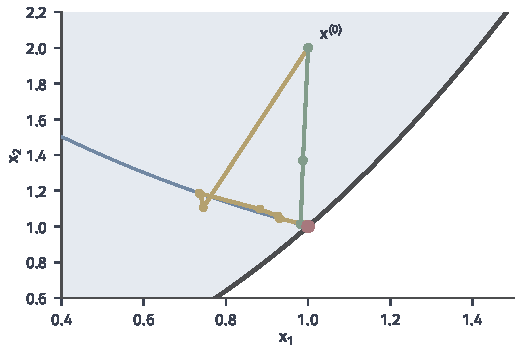
\includegraphics[width=88mm]{figures/05-optimization/06-constrained-optimization/matplotlib/nlipm-iterates/figure.pdf}
  \caption{贯穿例的迭代点，局部放大。蓝线是中心路径，绿线是$\sigma=0.2$的原始—对偶迭代，黄线是$\tau=0.2$的障碍法的Newton迭代点，红点是$\bm{x}^\star$，深灰粗线是约束边界。两者都从$(1,2)$出发。}
  \label{fig:nlipm-iterates}
\end{BookInlineFigure}

\begin{BookInlineFigure}
  \centering
  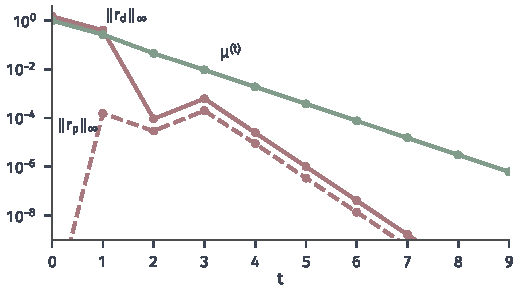
\includegraphics[width=88mm]{figures/05-optimization/06-constrained-optimization/matplotlib/nlipm-residual-curves/figure.pdf}
  \caption{贯穿例的残差历史，对数纵轴。红色实线是$\lVert\bm{r}_{\mathrm{d}}\rVert_\infty$，红色虚线是$\lVert\bm{r}_{\mathrm{p}}\rVert_\infty$（第$0$轮为零，图中从下方进入），绿线是$\mu^{(t)}$。}
  \label{fig:nlipm-residual-curves}
\end{BookInlineFigure}

\paragraph{预测—校正要重新核对条件}
第~\ref{chap:lp-interior-point}章的预测—校正可以直接搬用：先解$\sigma=0$的方程组，用试走后的互补量选$\sigma$，再把$\Delta s_i^{\mathrm{a}}\Delta\lambda_i^{\mathrm{a}}$移到右端。两次求解共用一次分解。例中第一轮，预测步的结果是
\[
 \alpha^{\mathrm{a}}\approx0.7015,\qquad\mu^{\mathrm{a}}\approx0.1640,\qquad\sigma\approx0.0044.
\]
校正后取到$\alpha\approx0.8556$，平均互补量降到$0.2085$，而固定$\sigma=0.2$时是$0.2673$。代价也很明显：两个乘积变成$0.0997$和$0.3174$，不再相等。

搬用时有三点要重新核对。校正项只补偿了互补方程的二阶项，约束的二阶余项$\bm{\rho}$并没有补偿。预测步用的$\bm{W}$若经过了正则化，二阶项的估计就是另一个问题的量。线性规划中单位步之后等式残差恰好消失，这里没有这个性质，所以校正之后的步长仍要过残差或过滤器的检验，单靠比例规则不够。
